\chapter{Introduction}
\label{ch:intro}

Modern media and news distribution is shifting from traditional media to social media.
Modern media production and information distribution is shifting from traditional outlets.
Also media consumption is shifting from traditional outlets to digital and mobile devices.
From con-sumer to pro-sumer.
News is not bound to expert opinion or an editorial news desk.
The opinion of the individual can be broad-casted without the need for a professional studio and equipment.
No office is required anymore to link a mobile eye-witness to a mass audience.

%What advantages does a smart phone have compared to a laptop and desktop?
Given this context mobile devices are increasingly important and smart-phone in particular.
A smart-phone has the unique property of being a ubiquitous device that is highly mobile and extremely connectible.
Most smart-phones even have one or more cameras to produce multi-media content that can be shared immediately from the device.
Finally the entire world has a smart-phone.
Even or especially areas without tradition infrastructure they are ubiquitous.

In crisis situations, like natural disaster or unrest, the smart-phone becomes particularly important, exactly for the earlier mentioned properties, as under such conditions utilizing centralized infrastructure is undesired (censorship) or physically impossible.
Decentralized can work in these situations.
Censorship and large scale monitoring is difficult in decentralized networks.
%REF article Johan 2011 voor voorbeeld


Tribler is a fully decentralized video-on-demand system. \cite{TriblerOverviewJournal, tribler2014play, tribler-anon-hd}
It is autonomous, attack-resilient and self-organizing. \cite{votecast, tribler-gossip}
It uses network overlays called communities to offer features like keyword search and managing contributions to channels for discover-ability of content.
It offers privacy through layered encrypted tunnels similar to the TOR network.\cite{triber2014at3, dingledine2004tor, dingledine2006design}

So far Tribler only supports desktop and server versions of Linux, Mac and Windows.
The necessity of moving to mobile devices calls for Tribler functionality to be enabled to run on these resource limited devices.
In this thesis the first prototype is presented that has all Tribler functionality fully enabled on mobile devices.
The prototype is build for Android OS since Android dominates the smart-phone market.
% maybe geographical spread of Android?



%% Shift to social media
% Production
Sharing opinion and discussion is enabled on social media.
A global dialog is possible through social media like Twitter, Instagram and Facebook.
% Consumption
People receive local and global news perceived relevant to their group on their social media feed.
Young people in particular are shifting to social media as their number one source. \cite{reuters_social_media}
As shown in this age distribution graph, figure \ref{fig:reuters-news-sources-ages}.
\begin{figure}[H]
	\centering
	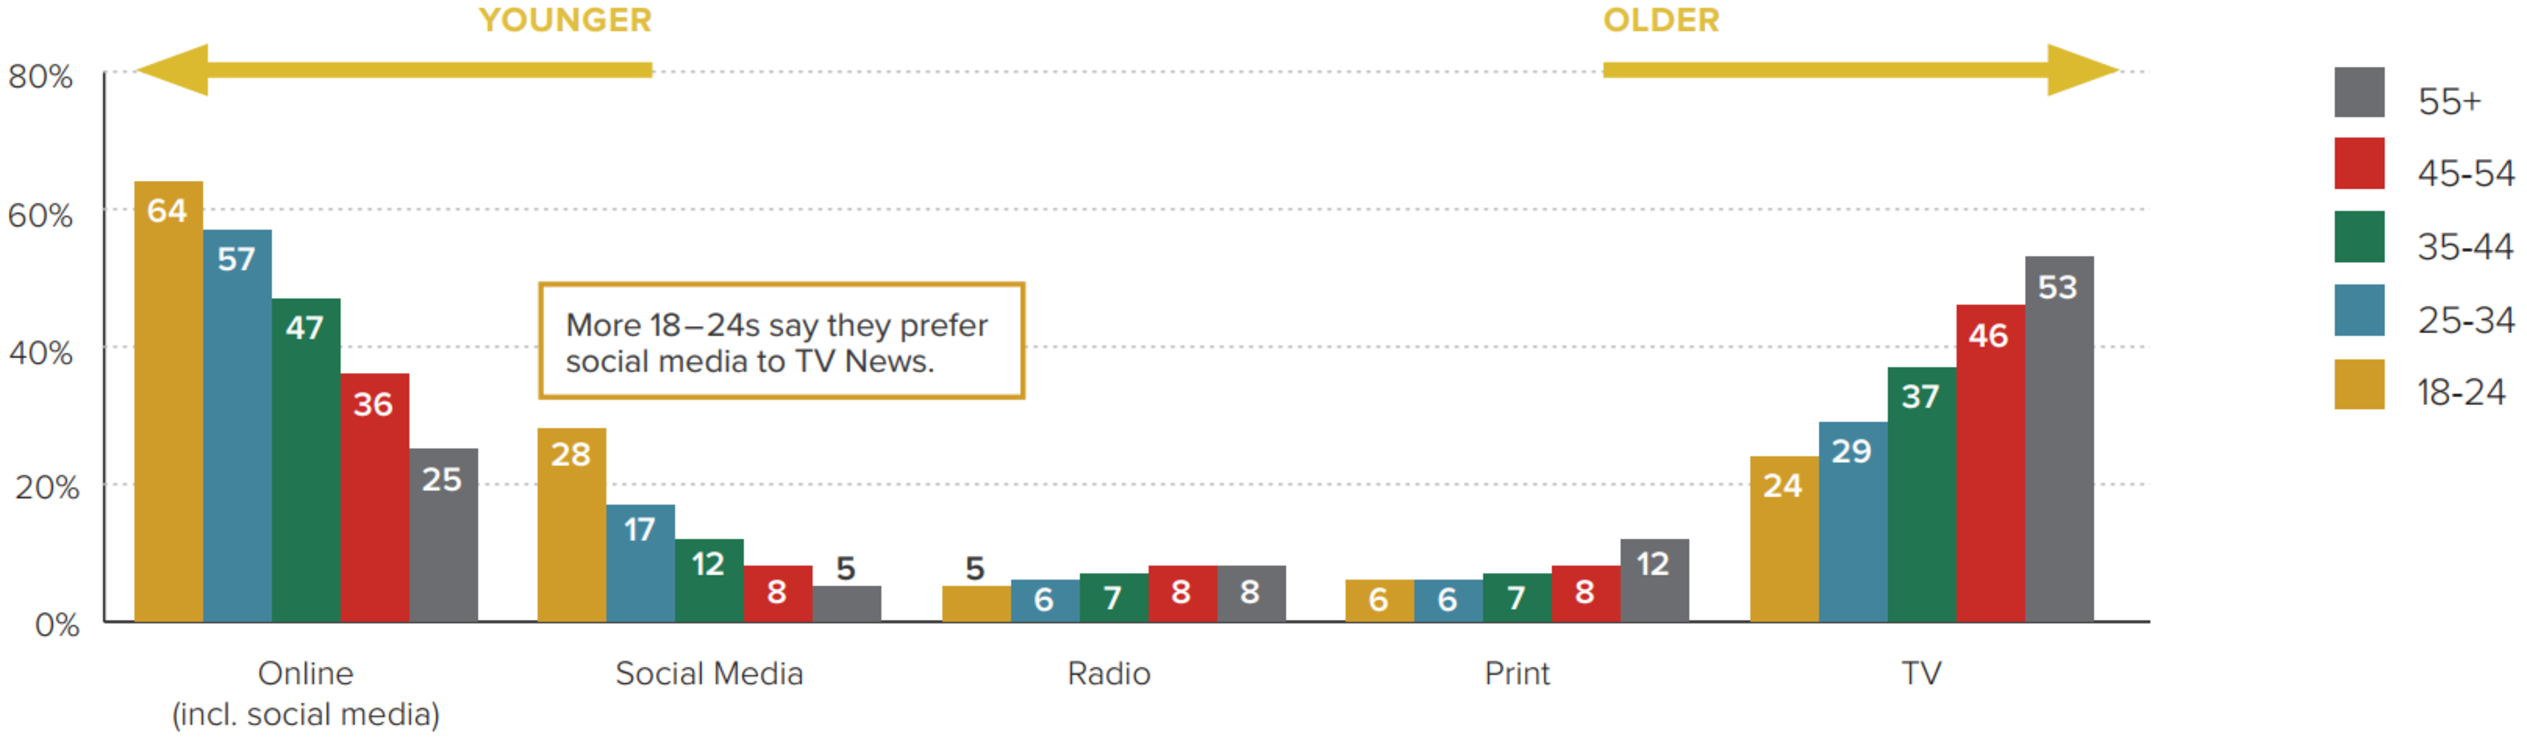
\includegraphics[width=\textwidth]{reuters-news-sources-ages}
	\caption{Main news sources split by age \cite{reuters_social_media}}
	\label{fig:reuters-news-sources-ages}
\end{figure}
% Distribution
Not only is social media more and more becoming a major distribution channel for news, it also starts delivering input for news and story creation.
This way social media has become both the source and outlet for investigative journalism.

%% Rise of the smart-phone
% Ubiquity
A smart-phone has the unique property of being a ubiquitous device that is highly mobile and extremely connectible.
Figure \ref{fig:smartphone-sales} shows that world-wide 1,4 billion smart-phones were sold to end-users last year.
And this number keeps rising.
Even or especially areas without traditional infrastructure they are ubiquitous.
\begin{figure}[H]
	\centering
	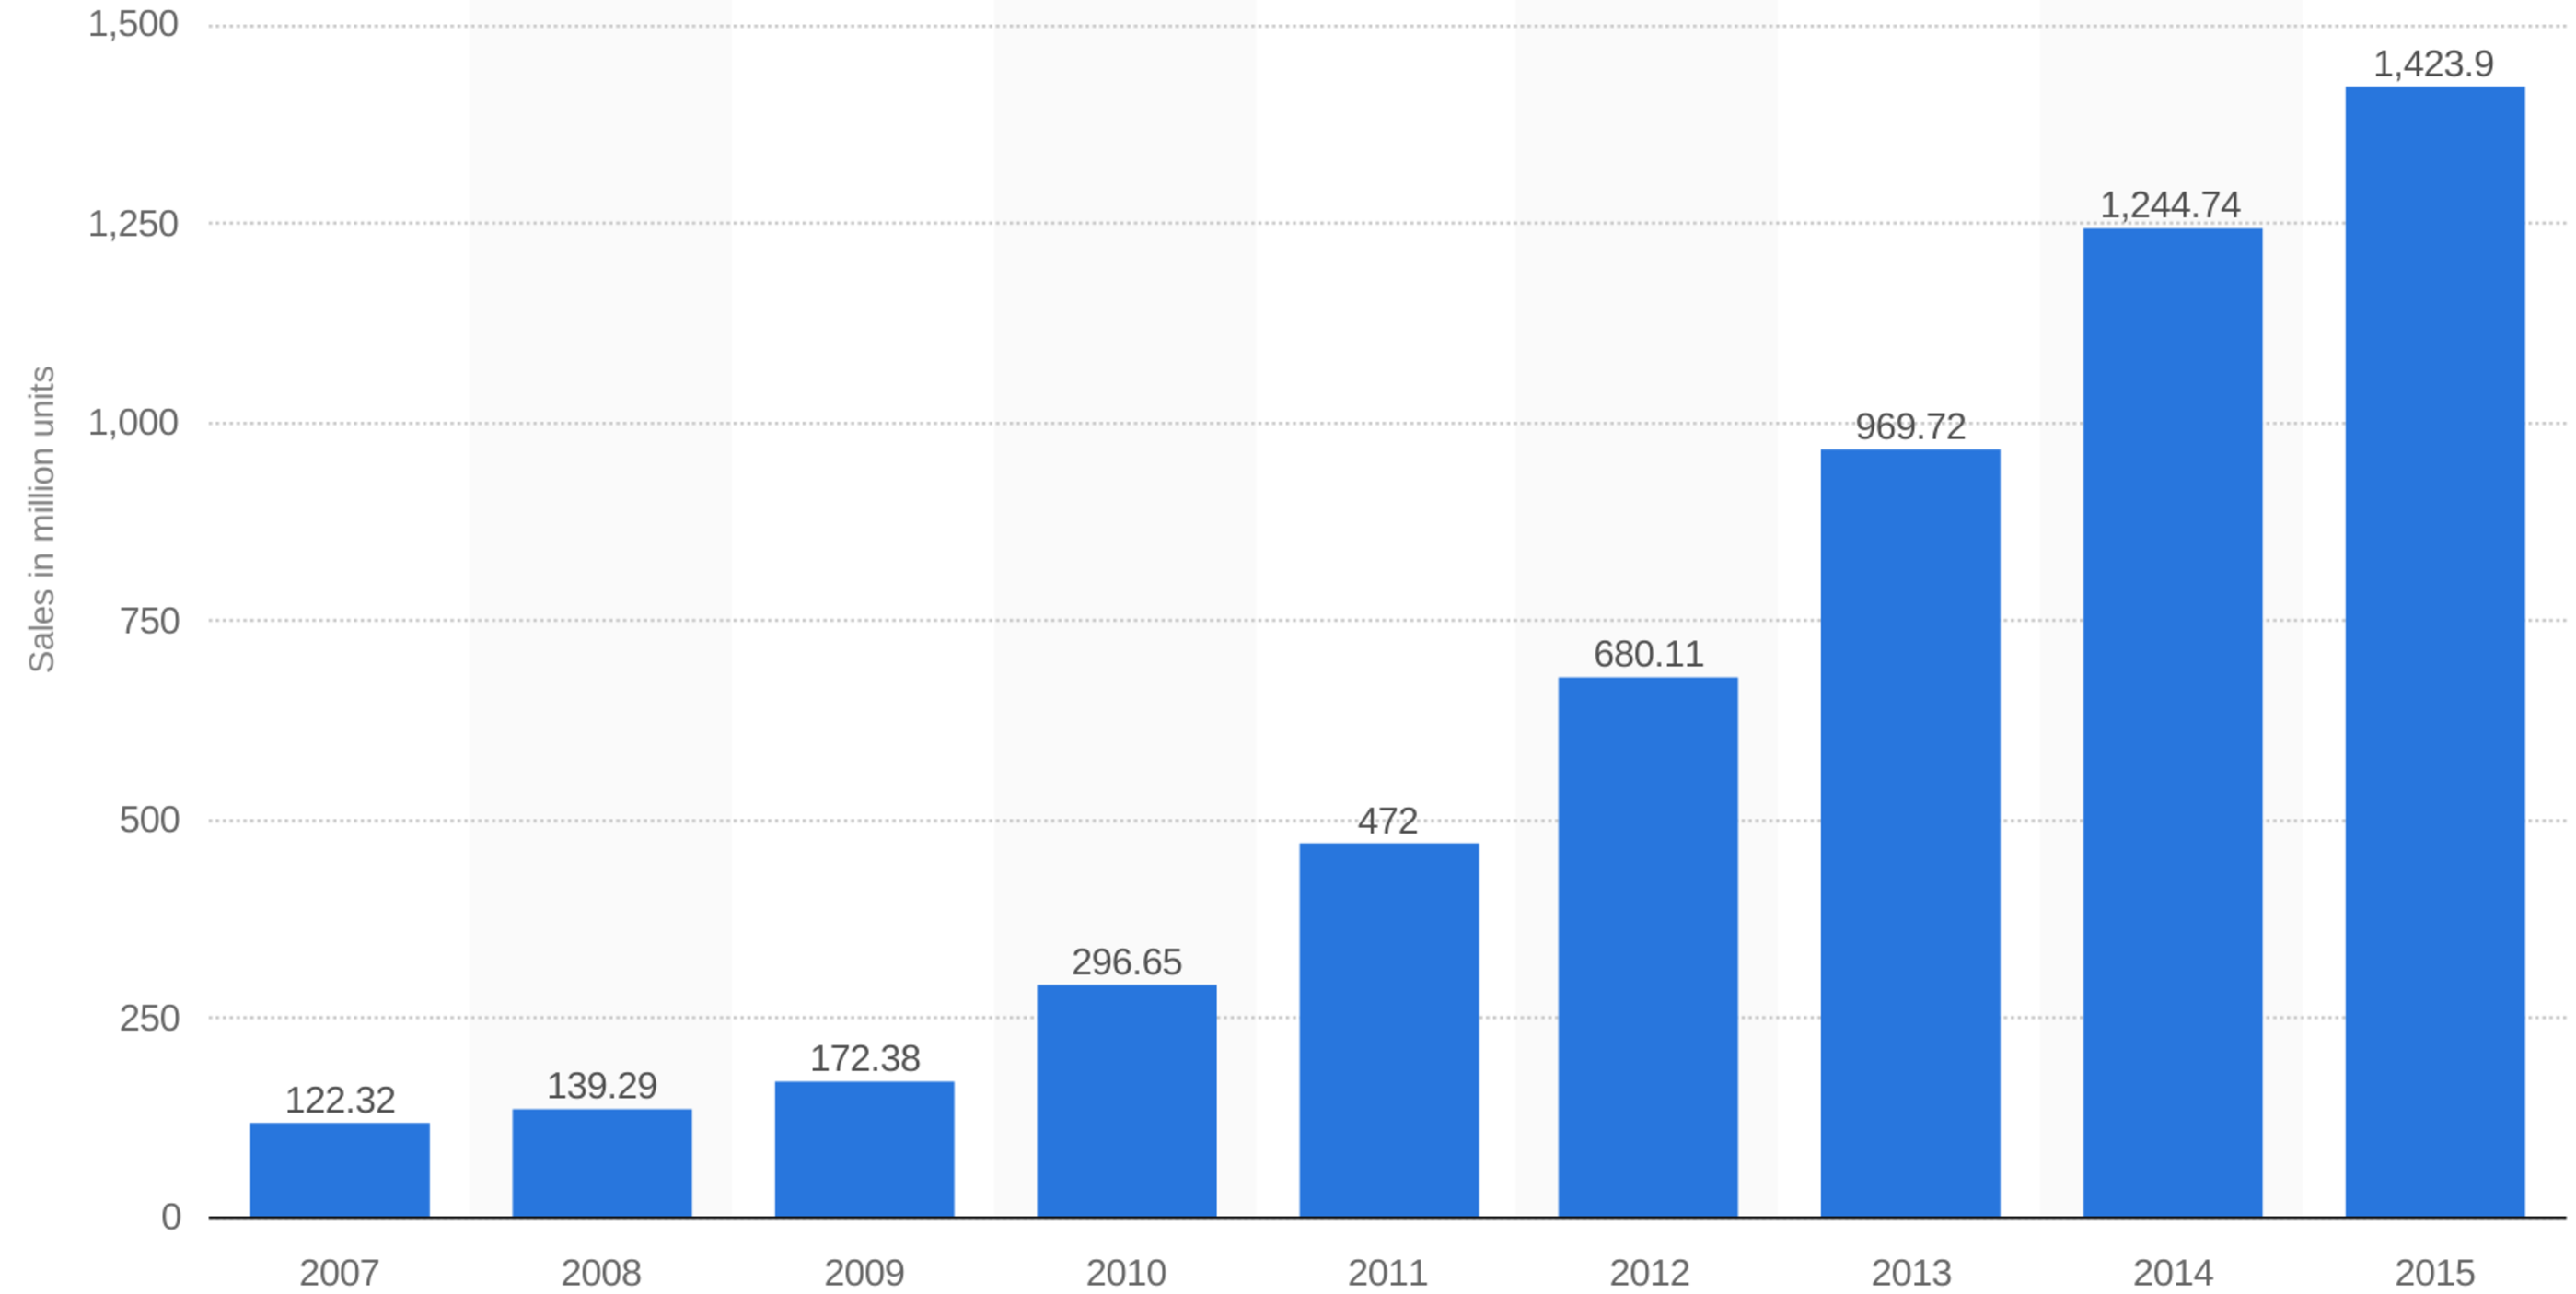
\includegraphics[width=\textwidth]{smartphone-sales}
	\caption{Number of smart-phones sold to end users worldwide from 2007 to 2015 (in million units) \cite{smartphone-sales}}
	\label{fig:smartphone-sales}
\end{figure}

The capabilities and versatility of smart-phones enable it to be used for production and consumption of news and social media.
The users themselves are turning from con-sumers into pro-sumers \cite{??}.
% Production
% Distribution
With regards to production most smart-phones have one or more cameras to record multi-media content that can be shared immediately from the device.
Eye-witnesses often have smart-phones at hand to immediately record an event with and post it on social media \cite{paris-attacks}.
No news desk or professional equipment is necessary to relay news directly from eye-witnesses to the masses anymore \cite{belgium-attacks}.
% Social journalism
People with camera phones can reach millions of people with multi-media in a very short timespan, becoming social journalists.
% Editorial / Journalism / Processing
The ease of reaching a global audience by an individual with a smart-phone diminishes the role of an expert curator handling incoming information.

% Consumption
Also with regard to the consumption medium mobile devices increasingly replace the role of traditional outlets like TV, newspapers and other physical media.

%% Communication during crisis
In crisis situations, like natural disaster or unrest, people need to communicate and coordinate their efforts to restore safety.
In this context the smart-phone becomes particularly important because it is often carried on person and provides connectability

In recent calamities \cite{earthquake-nepal, etc...} people could mark themselves as safe on social media, effectively broadcasting that information to all their family and friends on social media instead of contacting them one by one or not at all due to congestion in the communication channels.

However, several natural disasters have taken out the necessary infrastructure on numerous occasions for a prolonged period of time. %katrina

Therefore we require a solution to enable social media on smart-phones that does not require infrastructure. % persistent, established ??



%How to create a \emph{self-organising} \emph{video-on-demand} platform that is \emph{attack-resilient} and can \emph{operate autonomously} on a \emph{mobile device}?

The main research question is: how feasible is it to run all Tribler functionality on mobile devices? % to defeat or mitigate large scale monitoring and censorship?

Secondary question is: using the unique properties of mobile devices, what features can be added or enhanced?
Secondary question is: considering the constraints and opportunities of mobile devices, what unique ability can be utilized to extend or enhance Tribler?
